\documentclass[../AnalysisNoteJBuxton.tex]{subfiles}
\begin{document}

\section{Correlation Functions}
\label{CorrelationFunctions}

General remarks about formaton of correlation functions and what information they provide.

\begin{figure}[h]
  \centering
  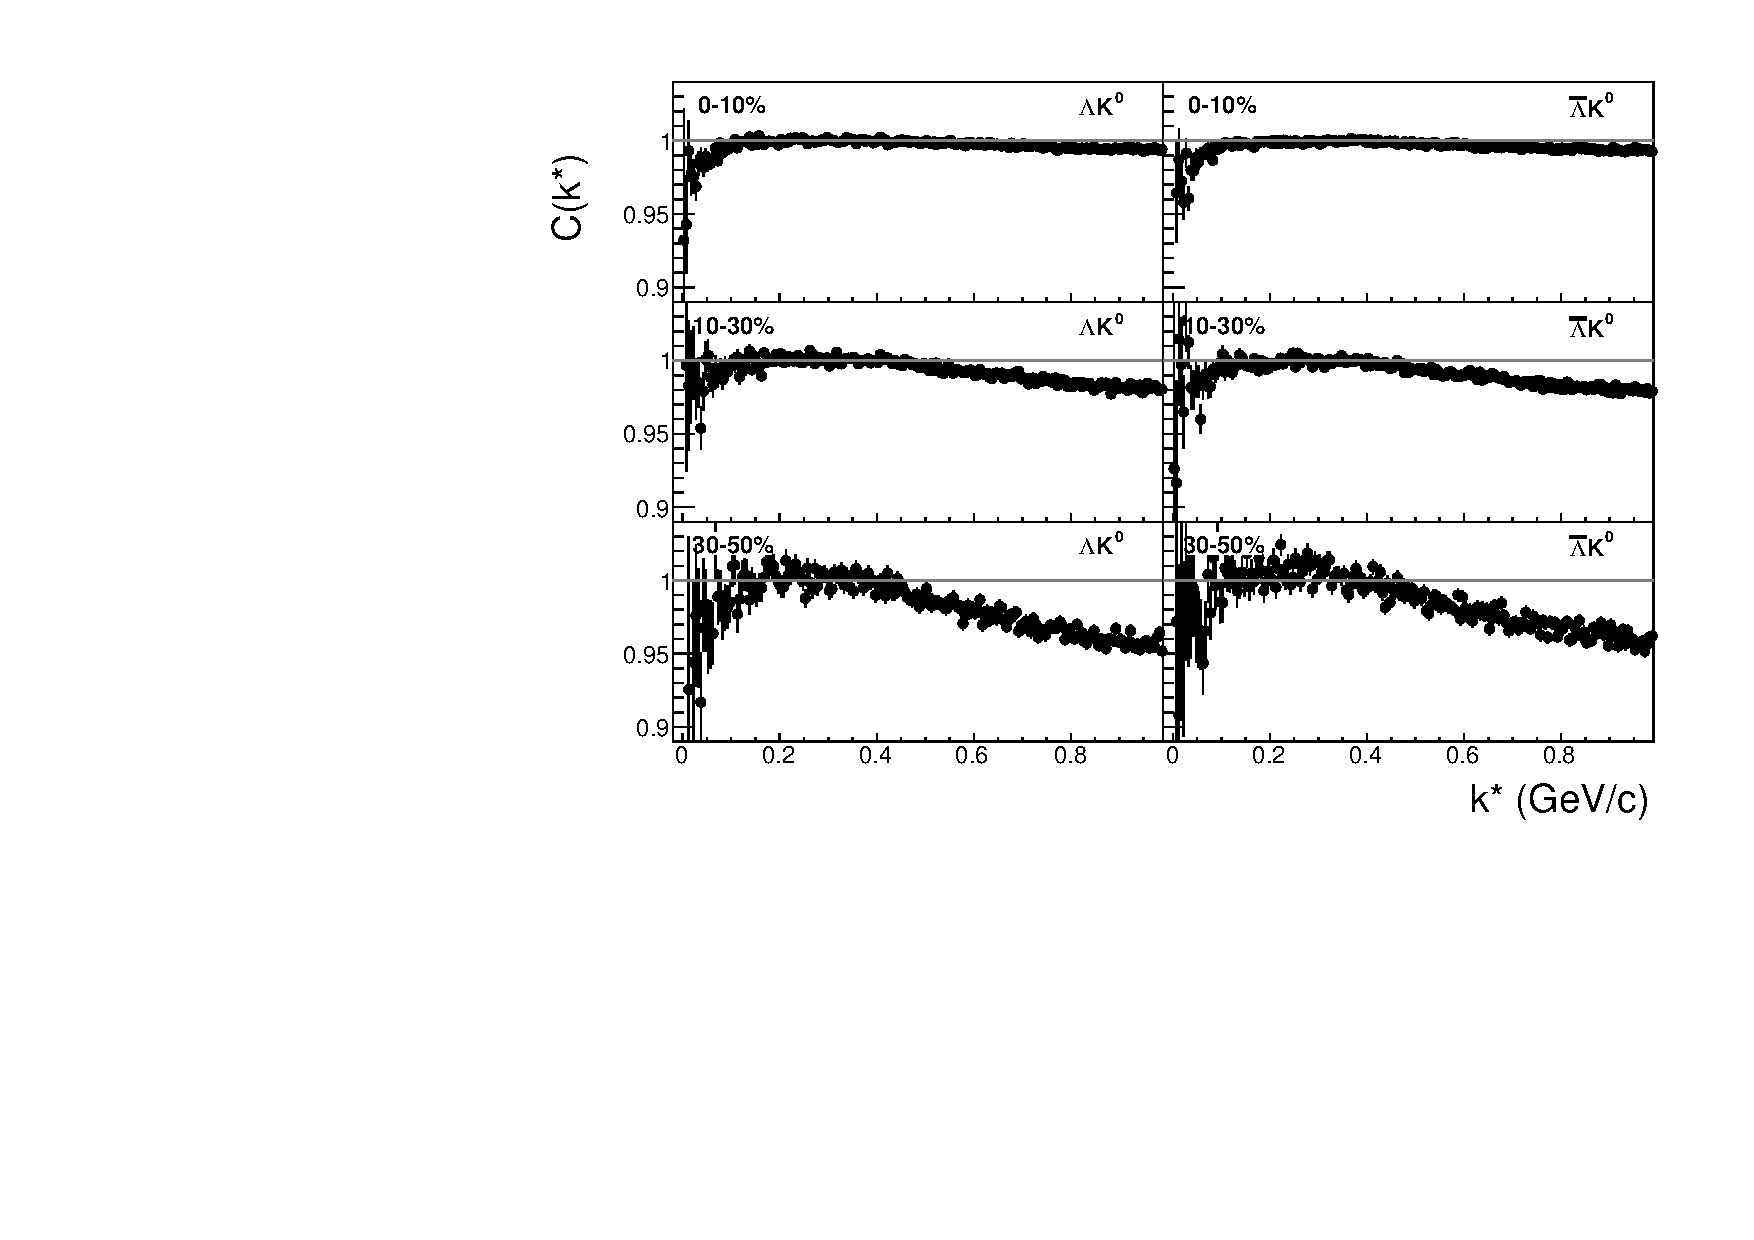
\includegraphics[width=\textwidth]{4_CorrelationFunctions/Figures/canKStarCfsLamK0wConj.pdf}
  \caption[$\Lambda$($\bar{\Lambda}$)K$^{0}_{S}$ Correlation Functions]{$\Lambda$K$^{0}_{S}$ (left) and $\bar{\Lambda}$K$^{0}_{S}$ (right) correlation functions for 0-10\% (top), 10-30\%(middle), and 30-50\%(bottom) centralities.}
  \label{fig:cLamK0Cfs}
\end{figure}

\begin{figure}[h]
  \centering
  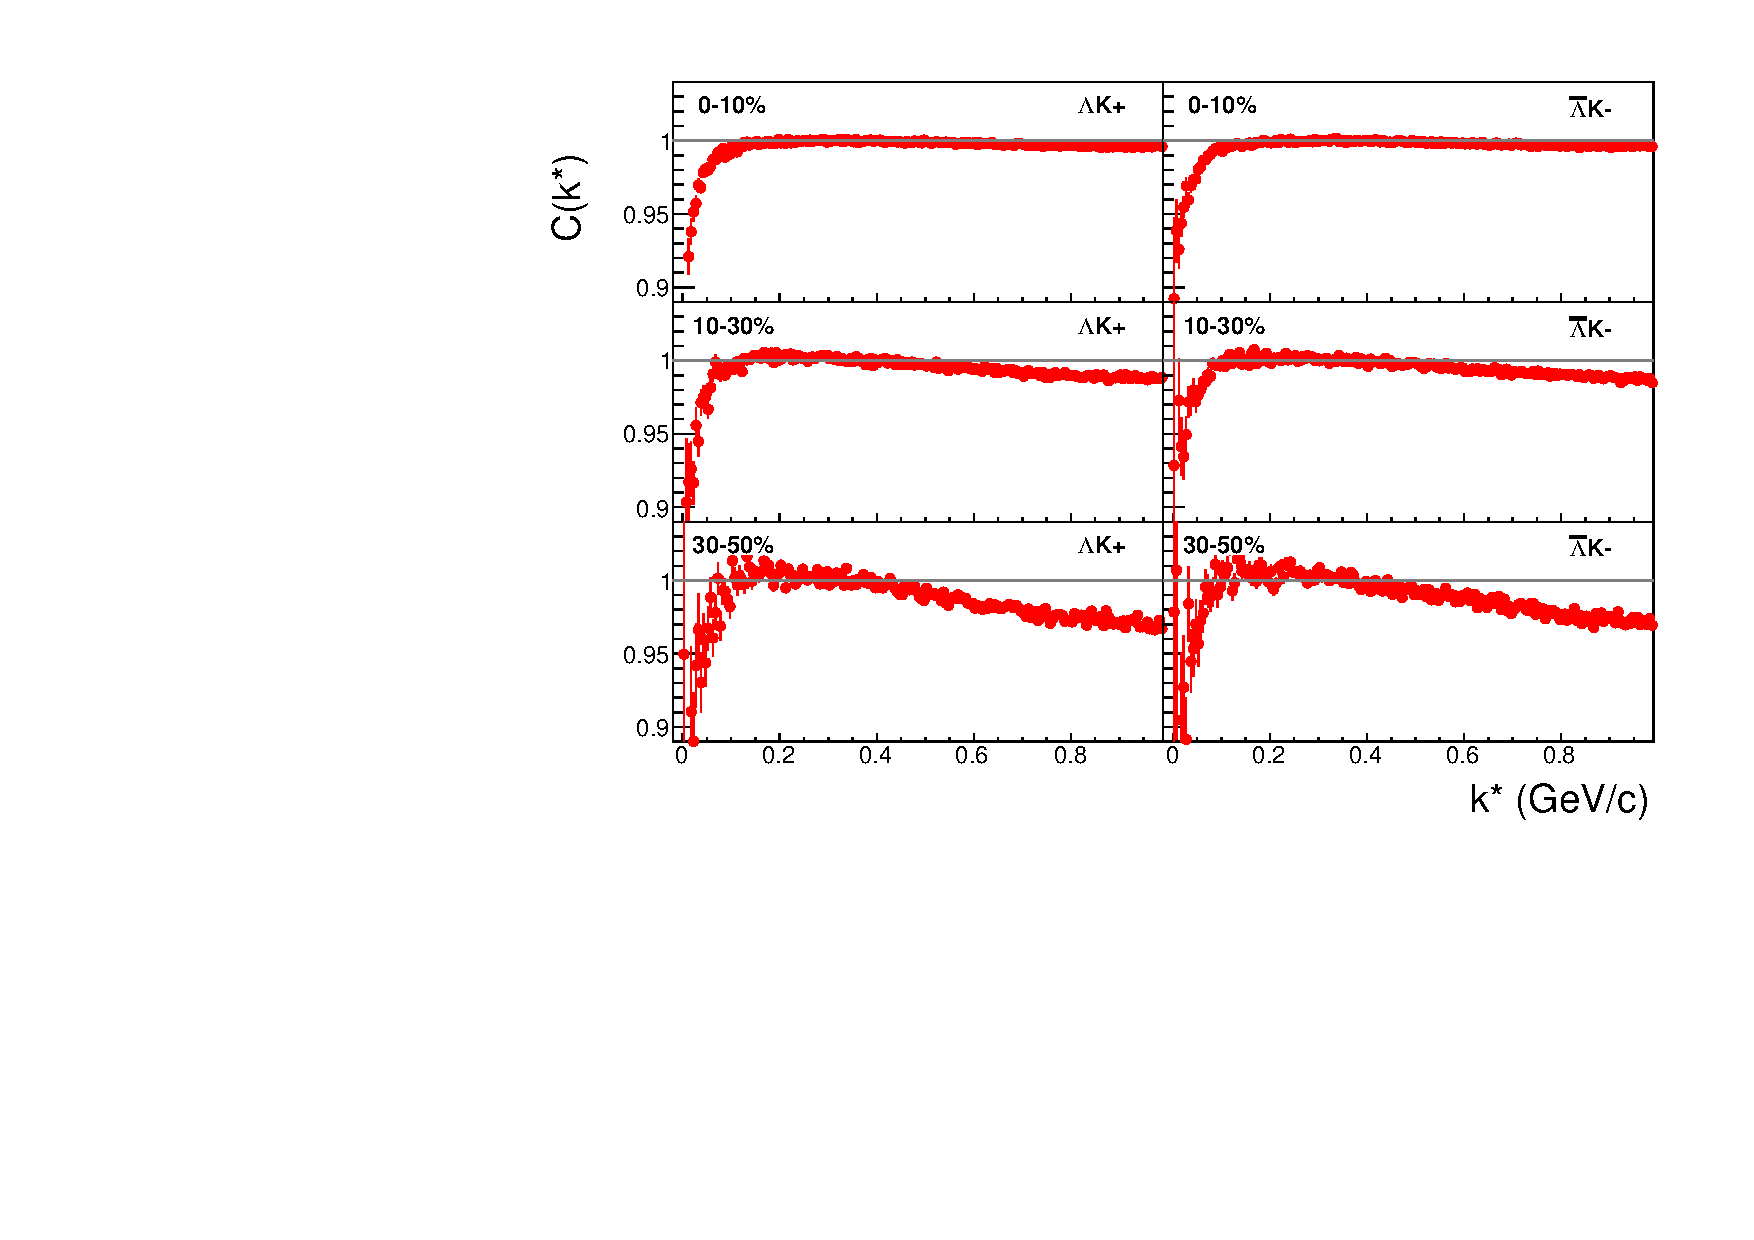
\includegraphics[width=\textwidth]{4_CorrelationFunctions/Figures/canKStarCfsLamKchPwConj.pdf}
  \caption[$\Lambda$K$^{+}$ and $\bar{\Lambda}$K$^{-}$ Correlation Functions]{$\Lambda$K$^{+}$ (left) and $\bar{\Lambda}$K$^{-}$ (right) correlation functions for 0-10\% (top), 10-30\%(middle), and 30-50\%(bottom) centralities.}
  \label{fig:LamKchPwConjCfs}
\end{figure}

\begin{figure}[h]
  \centering
  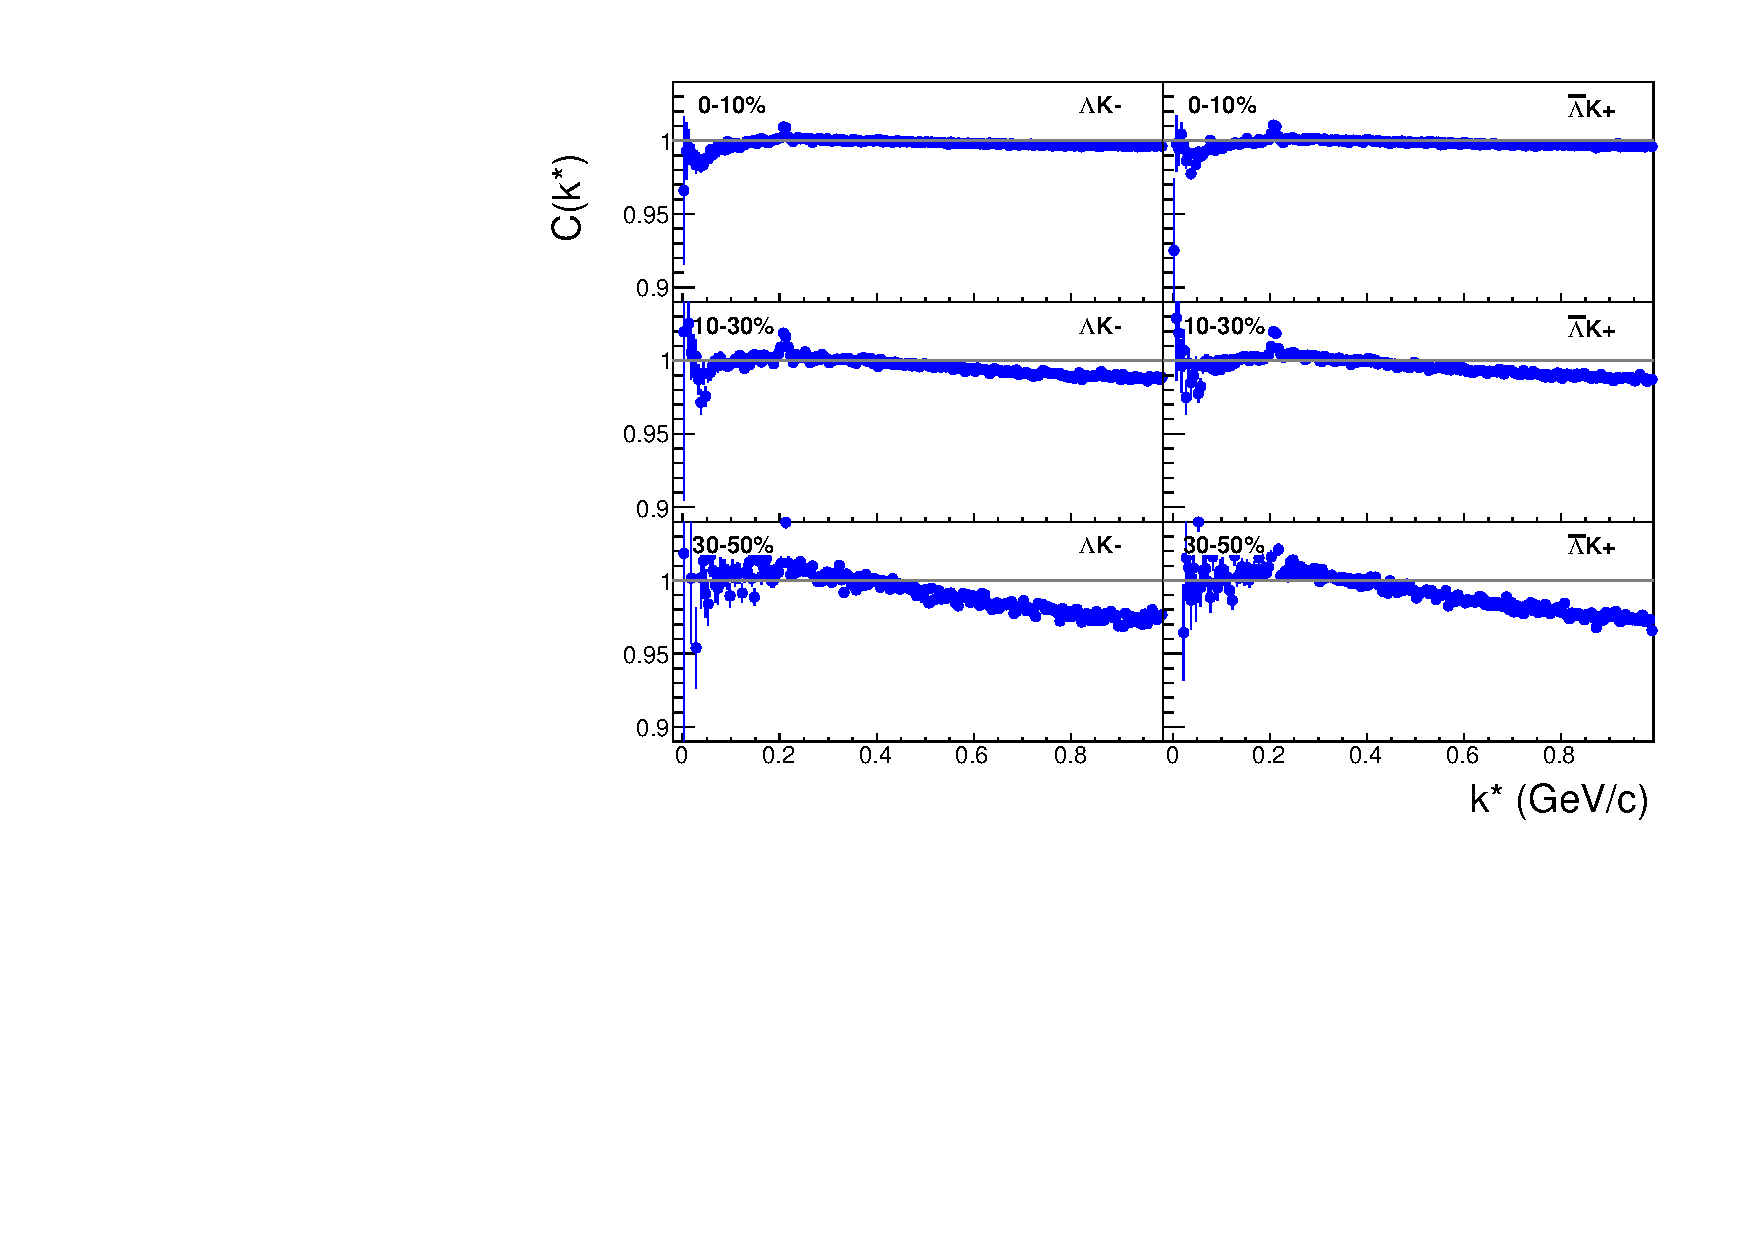
\includegraphics[width=\textwidth]{4_CorrelationFunctions/Figures/canKStarCfsLamKchMwConj.pdf}
  \caption[$\Lambda$K$^{-}$ and $\bar{\Lambda}$K$^{+}$ Correlation Functions]{$\Lambda$K$^{-}$ (left) and $\bar{\Lambda}$K$^{+}$ (right) correlation functions for 0-10\% (top), 10-30\%(middle), and 30-50\%(bottom) centralities.  The peak at k* $\approx$ 0.2 GeV/c is due to the $\Omega^{-}$ resonance.}
  \label{fig:LamKchMwConjCfs}
\end{figure}

\begin{figure}[h]
  \centering
  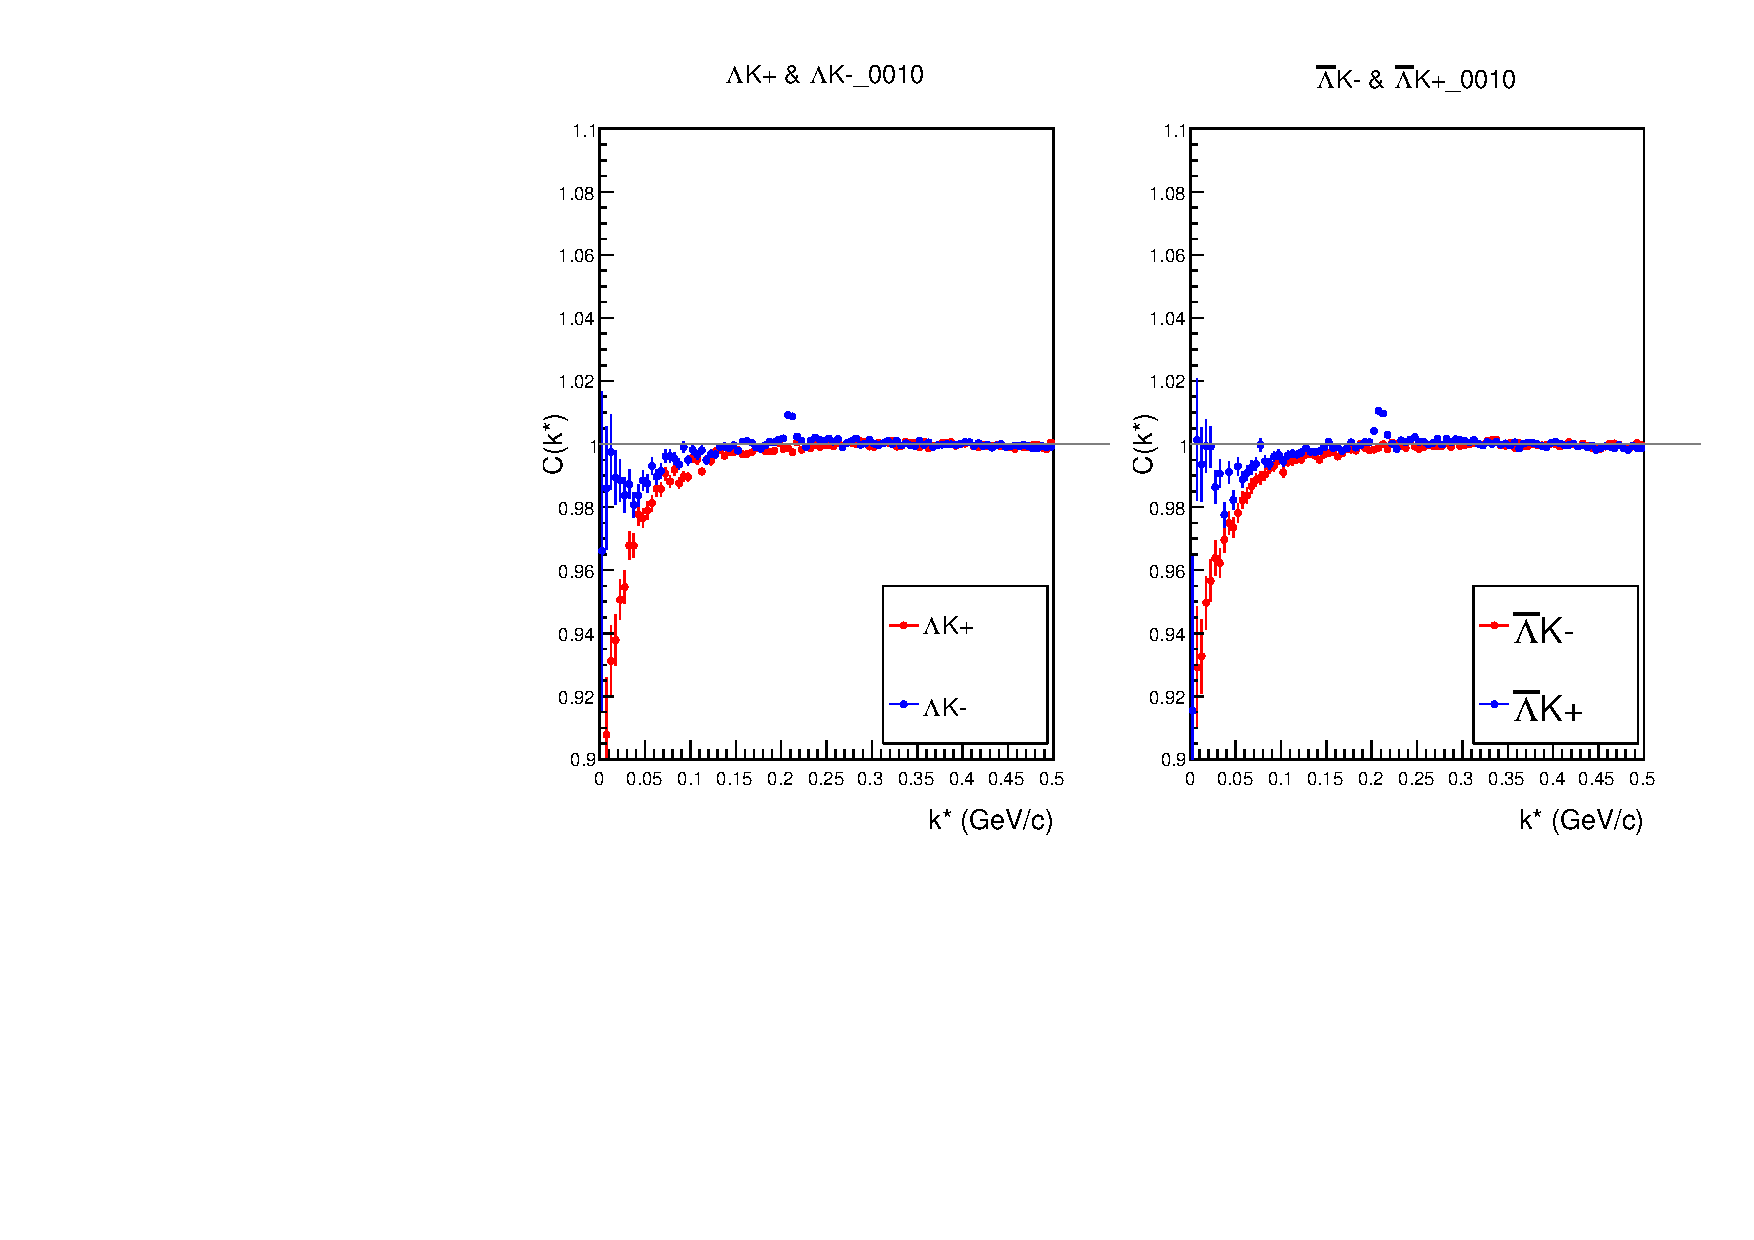
\includegraphics[width=\textwidth]{4_CorrelationFunctions/Figures/canKStarCfLamKchP_0010.pdf}
  \caption[Correlation Functions: $\Lambda$K$^{+}$ vs $\Lambda$K$^{-}$ for 0-10\% Centrality]{Correlation Functions: $\Lambda$K$^{+}$ vs $\Lambda$K$^{-}$ ($\bar{\Lambda}$K$^{+}$ vs $\bar{\Lambda}$K$^{-}$) for 0-10\% centrality.  The peak in $\Lambda$K$^{-}$($\bar{\Lambda}$K$^{+}$) at k* $\approx$ 0.2 GeV/c is due to the $\Omega^{-}$ resonance.}
  \label{fig:cLamcKchCfs0010}
\end{figure}

\end{document}